\documentclass[serif, aspectratio=169]{beamer}
%\documentclass[serif]{beamer}  % for 4:3 ratio

% Use XeLaTeX or LuaLaTeX for better font handling
\usepackage{fontspec} % For font selection
\usepackage{polyglossia} % For multilingual support
\setdefaultlanguage{vietnamese} % Set default language to Vietnamese
\setotherlanguage{english} % Add English as another language

% Set the main font to a font that supports Vietnamese characters
\newfontface\myfont{Times New Roman} % Change to your preferred font

\usepackage{hyperref}
\usepackage{graphicx}
\usepackage{amsmath}
\usepackage{multicol}
\usepackage{booktabs}
\usepackage{lipsum}


\usepackage{hyperref}


\usepackage{graphicx,pstricks,listings,stackengine}

\author{Nhóm 3}
\title{Phân loại thư rác sử dụng thuật toán SVM}
% \subtitle{Your Subtitle}
\institute{
	B22DCKH024 -	Vũ Công Tuấn Dương \\
	B22DCCN768 - Nguyễn Sơn Tùng \\
	B22DCCN479	- Nguyễn Đức Lâm \\
	B22DCCN347	- Trần Đức Hoàng \\
	B22DCCN348	- Trần Huy Hoàng \\
}
\date{\small \today}
\usepackage{HKUSTstyle}

% defs
\def\cmd#1{\texttt{\color{red}\footnotesize $\backslash$#1}}
\def\env#1{\texttt{\color{blue}\footnotesize #1}}
% set colors
\definecolor{hkustyellow}{RGB}{167, 131, 55}
\definecolor{hkustblue}{RGB}{0, 56, 116}
\definecolor{hkustred}{RGB}{209, 51, 59}


\lstset{
	basicstyle=\ttfamily\small,
	keywordstyle=\bfseries\color{deepblue},
	emphstyle=\ttfamily\color{deepred},    % Custom highlighting style
	stringstyle=\color{deepgreen},
	numbers=left,
	numberstyle=\small\color{halfgray},
	rulesepcolor=\color{red!20!green!20!blue!20},
	frame=shadowbox,
}

%- --- --- --- --- --- --- --- --- --- --- --- --- --- --- --- 
\begin{document}
	
	\begin{frame}
		\titlepage
		\vspace*{-0.6cm}
		
	\end{frame}
	
	\begin{frame}    
		\tableofcontents[sectionstyle=show,
		subsectionstyle=show/shaded/hide,
		subsubsectionstyle=show/shaded/hide]
	\end{frame}
	
	% Introduction --- --- --- --- --- --- --- --- --- --- --- --- 
	
	\section{Giới thiệu}
	\begin{frame}{Bộ dữ liệu}
		\frametitle<presentation>{Bộ dữ liệu}
		\begin{block}{Dữ liệu được lấy trên \href{https://www.kaggle.com/datasets/purusinghvi/email-spam-classification-dataset}{Kaggle}}
			\begin{itemize}
				\item Combined Spam Email CSV of 2007 TREC Public Spam Corpus and Enron-Spam Dataset
				\item  83446 bản ghi email bằng tiếng Anh được phân loại thành 2 nhãn là Spam và Non-spam trong đó số email spam: 43910 và số email ham:(không spam) là 39538
			\end{itemize}
		\end{block}
		% \begin{block}{Advantages of using \LaTeX ~with the beamer package:}
			% 	\begin{itemize}
				% 		\item very easy if the report is already written in \LaTeX
				% 		\item different themes which are usable in practice
				% 		\item possibility to create handouts using \emph{beamerarticle}
				% 	\end{itemize}
			% \end{block}
	\end{frame}
	
	\begin{frame}{Mục tiêu}
		
		\begin{itemize}
			\item Xây dựng được mô hình Linear SVM Hard Margin cơ bản để phân loại
			\item Đánh giá mô hình dựa trên các thang đo như độ chính xác và F1 score
			\item Demo được trên giao diện web
		\end{itemize}
		
	\end{frame}
	
	% Literature Review --- --- --- --- --- --- --- --- --- --- --- 
	\section{Lý thuyết}
	\subsection{Lý thuyết SVM}
	\subsubsection{Hàm mục tiêu của SVM}
	\begin{frame}{Hàm mục tiêu của SVM}
		\begin{itemize}
			\item Mục tiêu của SVM là tối ưu hóa khoảng cách giữa các điểm dữ liệu của hai lớp. 
			\item Hàm mục tiêu được xây dựng sao cho margin giữa hai lớp là lớn nhất, đồng thời đảm bảo rằng không có điểm nào bị sai phân loại.
		\end{itemize}
		
	\end{frame}
	
	\begin{frame}{Ảnh minh hoạ}
		\begin{figure}
			\centering
			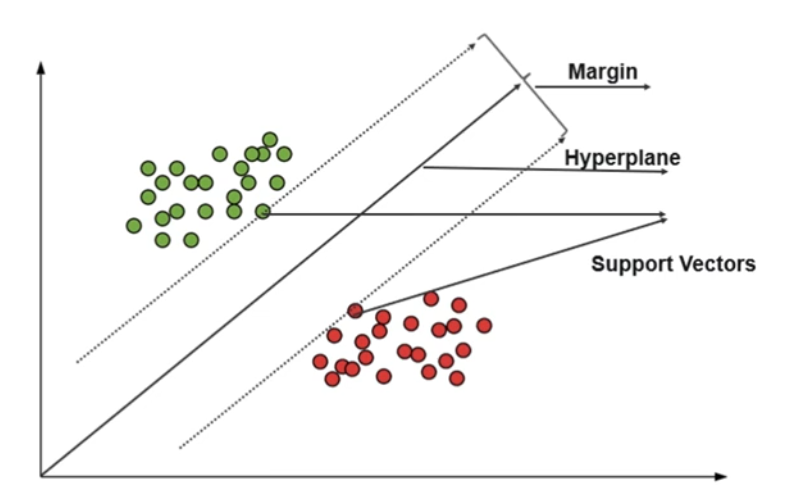
\includegraphics[height=5cm]{pic/svm.png}
			\caption{Mô tả thuật toán SVM}
			\label{fig:svm}
		\end{figure}
		
	\end{frame}
	
	
	\begin{frame}{Hàm mục tiêu của SVM}
		\begin{itemize}
			\item Nếu dữ liệu huấn luyện có thể phân tách tuyến tính, có thể chọn hai siêu phẳng song song để phân tách hai lớp dữ liệu, sao cho khoảng cách giữa chúng là lớn nhất có thể. 
			\item Khu vực được giới hạn bởi hai siêu phẳng này được gọi là "margin" (biên).Siêu phẳng có margin lớn nhất là siêu phẳng nằm ở giữa hai siêu phẳng này. 
		\end{itemize}
		
	\end{frame}
	
	\begin{frame}{Hàm mục tiêu của SVM}
		Với một bộ dữ liệu đã chuẩn hóa hoặc chuẩn hóa, các siêu phẳng này có thể được mô tả bằng các phương trình:
		\begin{itemize}
			\item \[
			\mathbf{w}^T \mathbf{x} + b = 1
			\]
			(mọi điểm trên hoặc phía trên ranh giới này thuộc về một lớp với nhãn 1)
			\item \[
			\mathbf{w}^T \mathbf{x} + b = -1
			\]
			(mọi điểm trên hoặc phía dưới ranh giới này thuộc về lớp còn lại, với nhãn -1).
		\end{itemize}
		Về mặt hình học, khoảng cách giữa 2 siêu phẳng này là \(\frac{2}{\| w \|}\) nên ta cần tối thiểu hóa \(\| w \|\). 
		
	\end{frame}
	
	\begin{frame}{Ràng buộc hàm mục tiêu}
		Cũng cần ngăn không cho các điểm dữ liệu rơi vào margin, vì vậy phải thêm vào ràng buộc sau: với mỗi \(i\), nếu \(y_i = 1\), thì phải có:
		
		\[
		w^T x_i + b \geq 1
		\]
		
		hoặc nếu \(y_i = -1\), thì phải có:
		
		\[
		w^T x_i + b \leq -1
		\]
		
		Ràng buộc này yêu cầu mỗi điểm dữ liệu phải nằm ở phía đúng của margin. Hay có thể viết lại là: \[
		y_i (w^T x_i + b) \geq 1, \quad \forall 1 \leq i \leq n
		\]
		
	\end{frame}
	
	\begin{frame}{Bài toán tối ưu}
		Tóm lại, ta cần giải bài toán tối ưu: \[
		\min_{w, b} \frac{1}{2} \| w \|^2
		\]
		
		với ràng buộc:
		
		\[
		y_i (w^T x_i + b) \geq 1 \quad \forall i \in \{1, \dots, n\}
		\]
		Cần tìm w và b
	\end{frame}
	\subsubsection{Phương trình Lagrange và điều kiện KKT}
	\begin{frame}{Hàm Lagrange}
		\[
		\mathcal{L}(w, b, \lambda) = \frac{1}{2} \| w \|^2 - \sum_{i=1}^{N} \lambda_i \left( y_i (w \cdot x_i + b) - 1 \right)
		\]
		\( \lambda_i \geq 0 \) là các hệ số Lagrange
	\end{frame}
	
	\begin{frame}{Điều kiện KKT}
		\begin{align*}
			& \lambda_i \geq 0 \quad \forall i=1,\ldots,n \quad\\
			& y^{(i)}(\mathbf{w} \cdot \mathbf{x}^{(i)} + b) - 1 \geq 0 \quad \forall i=1,\ldots,n \quad\\
			& \lambda_i [y^{(i)}(\mathbf{w} \cdot \mathbf{x}^{(i)} + b) - 1] = 0 \quad \forall i=1,\ldots,n \quad 
		\end{align*}
	\end{frame}
	
	\begin{frame}{Phương trình Lagrange và điều kiện KKT}
		\begin{itemize}
			\item \forall{i} : $\lambda_i = 0$ hoặc $y^{(i)}(\mathbf{w} \cdot \mathbf{x}^{(i)} + b) = 1$.
			\item Các điểm sao cho $\lambda_i > 0$ nằm trên margin được gọi là các vector hỗ trợ(support vectors)
			
		\end{itemize}
	\end{frame}
	\begin{frame}{Điều kiện KKT}
		\begin{align}
			\frac{\partial \mathcal{L}}{\partial \mathbf{w}} &= \mathbf{w} - \sum_{i=1}^{n} \lambda_i y^{(i)} \mathbf{x}^{(i)} = \mathbf{0} \\
			\frac{\partial \mathcal{L}}{\partial b} &= - \sum_{i=1}^{n} \lambda_i y^{(i)} = 0
		\end{align}
		Từ (1): \begin{equation}
			\mathbf{w} = \sum_{i=1}^{n} \lambda_i y^{(i)} \mathbf{x}^{(i)}
		\end{equation}
		Từ (2): \begin{equation}
			\sum_{i=1}^{n} \lambda_i y^{(i)} = 0
		\end{equation}
	\end{frame}
	
	\begin{frame}{Điều kiện KKT}
		\begin{align*} 
			L(\bm{w}, b, \lambda_1, \dots, \lambda_n) &\equiv \frac{1}{2}\|\bm{w}\|^2 - \sum_{i=1}^n \lambda_i \{ y^{(i)} (\bm{w}^{\top} \bm{x}^{(i)} + b) - 1 \} \\
			&= \frac{1}{2}\|\bm{w}\|^2 - \underbrace{\sum_{i=1}^n \lambda_i y^{(i)} \bm{x}^{(i)\top}}_{=\bm{w}^{\top}} \bm{w} - \underbrace{\sum_{i=1}^n\lambda_i y^{(i)}}_{=0} b + \sum_{i=1}^n \lambda_i 
		\end{align*}
	\end{frame}
	
	\begin{frame}{Điều kiện KKT}
		\begin{align*}
			L(\bm{w}, b, \lambda_1, \dots, \lambda_n) &\equiv \frac{1}{2}\|\bm{w}\|^2 -\| \bm{w} \|^2 + \sum_{i=1}^n \lambda_i \\
			&= \sum_{i=1}^n \lambda_i -\frac{1}{2}\|\bm{w}\|^2 \\
			&= \sum_{i=1}^n \lambda_i - \frac{1}{2} \sum_{i=1}^{n} \sum_{j=1}^{n} \lambda_{i} \lambda_{j} y^{(i)} y^{(j)}\bm{x}^{(i)\top}\bm{x}^{(j)} \\
			&\equiv \tilde{L}(\lambda_1, \dots, \lambda_n) \label{eq:L_tilde}
		\end{align*}
	\end{frame}
	
	\begin{frame}{Quy về bài toán}
		Có thể quy về bài toán tìm:
		\begin{align*}
			\hat{\lambda} &= \arg\max_{\lambda} \tilde{L}(\lambda) \\
			&= \arg\max_{\lambda} \left\{\sum_{i=1}^n \lambda_i - \frac{1}{2}\sum_{i=1}^n \sum_{j=1}^n \lambda_i \lambda_j y^{(i)}y^{(j)}\mathbf{x}^{(i)T}\mathbf{x}^{(j)}\right\} \\
			&\text{với điều kiện } \lambda_i \geq 0, \sum_{i=0}^n \lambda_i y^{(i)} = 0, (i=1,2,\ldots,n).
		\end{align*}
	\end{frame}
	\subsubsection{Ước lượng $\hat{\lambda}$}
	\begin{frame}{Ước lượng $\hat{\lambda}$ bằng phương pháp Gradient Descent}
		\begin{block}{Nguyên lý phương pháp}
			\begin{itemize}
				\item Phương pháp Gradient Descent được sử dụng để tìm nghiệm tối ưu $\hat{\lambda}$
				\item Các giá trị tham số ban đầu $\lambda^{[0]}$ được đặt ngẫu nhiên
				\item Cập nhật theo hướng gradient (vì đây là bài toán tối đa hóa):
				\[\bm{\lambda}^{[t+1]} = \bm{\lambda}^{[t]} + \eta \pd{\tilde{L}(\bm{\lambda})}{\bm{\lambda}}\]
				\item $\eta$ là tốc độ học (learning rate)
			\end{itemize}
		\end{block}
	\end{frame}
	
	\begin{frame}{Biểu diễn vector cho bài toán SVM}
		\begin{block}{Ma trận dữ liệu và vector}
			\begin{align*}
				\mathbf{X}_{[n \times p]} &= 
				\begin{pmatrix}
					x^{(1)}_1 & x^{(1)}_2 & \cdots & x^{(1)}_p \\
					x^{(2)}_1 & x^{(2)}_2 & \cdots & x^{(2)}_p \\
					\vdots & \vdots & \ddots & \vdots \\
					x^{(n)}_1 & x^{(n)}_2 & \cdots & x^{(n)}_p
				\end{pmatrix}
				=
				\begin{pmatrix}
					- \mathbf{x}^{(1)T} - \\
					- \mathbf{x}^{(2)T} - \\
					\vdots \\
					- \mathbf{x}^{(n)T} -
				\end{pmatrix} \\
				\mathbf{y}_{[n \times 1]} &= 
				\begin{pmatrix}
					y^{(1)} \\
					y^{(2)} \\
					\vdots \\
					y^{(n)}
				\end{pmatrix},
				\quad
				\bm{\lambda}_{[n \times 1]} = 
				\begin{pmatrix}
					\lambda_1 \\
					\lambda_2 \\
					\vdots \\
					\lambda_n
				\end{pmatrix}
			\end{align*}
		\end{block}
	\end{frame}
	
	\begin{frame}{Ma trận H và phép nhân Hadamard}
		\begin{block}{Định nghĩa ma trận H}
			\begin{align*}
				\mathbf{H}_{[n \times n]} &\equiv \mathbf{y}_{[n \times 1]} \mathbf{y}^T_{[1 \times n]} \odot \mathbf{X}_{[n \times p]} \mathbf{X}^T_{[p \times n]}
			\end{align*}
			\begin{itemize}
				\item $\odot$ là tích Hadamard (phép nhân từng phần tử)
				\item Các phần tử của ma trận: $(H)_{ij} = y^{(i)}y^{(j)}\mathbf{x}^{(i)T}\mathbf{x}^{(j)}$
				\item H là ma trận đối xứng
			\end{itemize}
		\end{block}
	\end{frame}
	
	\begin{frame}{Viết lại hàm Lagrangian}
		\begin{block}{Biểu diễn hàm Lagrangian dưới dạng vector}
			\begin{align*}
				\tilde{L}(\bm{\lambda}) &\equiv \sum_{i=1}^n \lambda_i - \frac{1}{2}\sum_{i=1}^n \sum_{j=1}^n \lambda_i \lambda_j y^{(i)}y^{(j)}\mathbf{x}^{(i)T}\mathbf{x}^{(j)} \\
				&= \sum_{i=1}^n \lambda_i - \frac{1}{2}\sum_{i=1}^n \sum_{j=1}^n \lambda_i \lambda_j (H)_{ij} \\
				&= \| \bm{\lambda} \| - \frac{1}{2}\bm{\lambda}^T H \bm{\lambda}
			\end{align*}
			Với $\| \bm{\lambda} \| = \sum_{i=1}^n \lambda_i$ là tổng các phần tử của vector $\bm{\lambda}$
		\end{block}
	\end{frame}
	
	\begin{frame}{Tính toán vector gradient}
		\begin{block}{Đạo hàm của hàm Lagrangian theo $\bm{\lambda}$}
			\begin{align*}
				\pd{\tilde{L}(\bm{\lambda})}{\bm{\lambda}} &= \pd{}{\bm{\lambda}} \| \bm{\lambda} \| - \frac{1}{2} \pd{}{\bm{\lambda}} \bm{\lambda}^T H \bm{\lambda} \\
				&= \mathbf{1} - H \bm{\lambda}
			\end{align*}
			Trong đó $\mathbf{1}$ là vector cột với tất cả các thành phần bằng 1:
			$\mathbf{1} = (1, 1, \ldots, 1)^T$
		\end{block}
	\end{frame}
	
	\begin{frame}{Quy tắc cập nhật trong Gradient Descent}
		\begin{block}{Quy tắc cập nhật cho nhân tử $\lambda$}
			\begin{align*}
				\bm{\lambda}^{[t+1]} = \bm{\lambda}^{[t]} + \eta(\mathbf{1} - H\bm{\lambda}^{[t]})
			\end{align*}
		\end{block}
		\begin{itemize}
			\item Cập nhật này được lặp đi lặp lại cho đến khi hội tụ
			\item Cần đảm bảo ràng buộc $\lambda_i \geq 0$ bằng cách cắt giá trị âm về 0
		\end{itemize}
	\end{frame}
	\subsubsection{Tìm $\hat{\mathbf{w}}$ và $\hat{b}$}
	\begin{frame}{Tìm $\hat{\mathbf{w}}$ từ $\hat{\lambda}$}
		\begin{block}{Tính vector trọng số $\hat{\mathbf{w}}$}
			Từ điều kiện KKT, ta có:
			\begin{align*}
				\hat{\mathbf{w}} = \sum_{i=1}^n \hat{\lambda}_i y^{(i)} \mathbf{x}^{(i)}
			\end{align*}
		\end{block}
		\begin{itemize}
			\item Từ điều kiện KKT (3):
			\begin{align*}
				\hat{\lambda}_i = 0, \text{ hoặc } y^{(i)}(\mathbf{w}^T \mathbf{x}^{(i)} + b) - 1 = 0
			\end{align*}
			\item Dữ liệu $\mathbf{x}^{(i)}$ được phân loại:
			\begin{align*}
				\begin{cases}
					\hat{\lambda}_i \neq 0 \Leftrightarrow \mathbf{x}^{(i)} \text{ là vector hỗ trợ}, \\
					\hat{\lambda}_i = 0 \Leftrightarrow \mathbf{x}^{(i)} \text{ không phải là vector hỗ trợ}.
				\end{cases}
			\end{align*}
		\end{itemize}
	\end{frame}
	
	\begin{frame}{Tìm $\hat{\mathbf{w}}$ từ $\hat{\lambda}$}
		\begin{block}{Tính vector trọng số $\hat{\mathbf{w}}$}
			Từ điều kiện KKT, ta có:
			\begin{align*}
				\hat{\mathbf{w}} = \sum_{i=1}^n \hat{\lambda}_i y^{(i)} \mathbf{x}^{(i)}
			\end{align*}
		\end{block}
		\begin{itemize}
			\item Chỉ tính tổng trên các vector hỗ trợ:
			\begin{align*}
				\hat{\mathbf{w}} = \sum_{\mathbf{x}^{(i)} \in S} \hat{\lambda}_i y^{(i)} \mathbf{x}^{(i)}
			\end{align*}
		\end{itemize}
	\end{frame}
	
	\begin{frame}{Tìm $\hat{b}$ từ các vector hỗ trợ}
		\begin{block}{Tính tham số $\hat{b}$}
			\begin{align*}
				\hat{b} &= \frac{1}{y^{(i)}} - \hat{\mathbf{w}}^T \mathbf{x}^{(i)} \\
				&= y^{(i)} - \hat{\mathbf{w}}^T \mathbf{x}^{(i)} \quad (\text{vì } y^{(i)} = 1 \text{ hoặc } -1)
			\end{align*}
		\end{block}
		\begin{itemize}
			\item Trong thực tế, để giảm sai số, tính trung bình trên tất cả các vector hỗ trợ:
			\begin{align*}
				\hat{b} = \frac{1}{|S|} \sum_{\mathbf{x}^{(i)} \in S} (y^{(i)} - \hat{\mathbf{w}}^T \mathbf{x}^{(i)})
			\end{align*}
			\item $|S|$ là số lượng vector hỗ trợ
		\end{itemize}
	\end{frame}
	
	\begin{frame}{Tóm tắt thuật toán Gradient Descent cho SVM}
		\begin{enumerate}
			\item \textbf{Khởi tạo:} $\lambda^{[0]}$ ngẫu nhiên, tính ma trận $H$
			\item \textbf{Lặp:} Cập nhật $\lambda$ theo công thức:
			\begin{align*}
				\bm{\lambda}^{[t+1]} = \bm{\lambda}^{[t]} + \eta(\mathbf{1} - H\bm{\lambda}^{[t]})
			\end{align*}
			\item \textbf{Áp dụng ràng buộc:} $\lambda_i \geq 0$
			\item \textbf{Tìm vector hỗ trợ:} $S = \{i : \lambda_i > 0\}$
			\item \textbf{Tính tham số mô hình:}
			\begin{align*}
				\hat{\mathbf{w}} &= \sum_{\mathbf{x}^{(i)} \in S} \hat{\lambda}_i y^{(i)} \mathbf{x}^{(i)} \\
				\hat{b} &= \frac{1}{|S|} \sum_{\mathbf{x}^{(i)} \in S} (y^{(i)} - \hat{\mathbf{w}}^T \mathbf{x}^{(i)})
			\end{align*}
		\end{enumerate}
	\end{frame}
	
	\subsection{Thuật toán Pegasos}
	\subsubsection{Thuật toán Pegasos cơ bản}
	\begin{frame}{Mô tả bằng mã giả}
		\begin{figure}
			\centering
			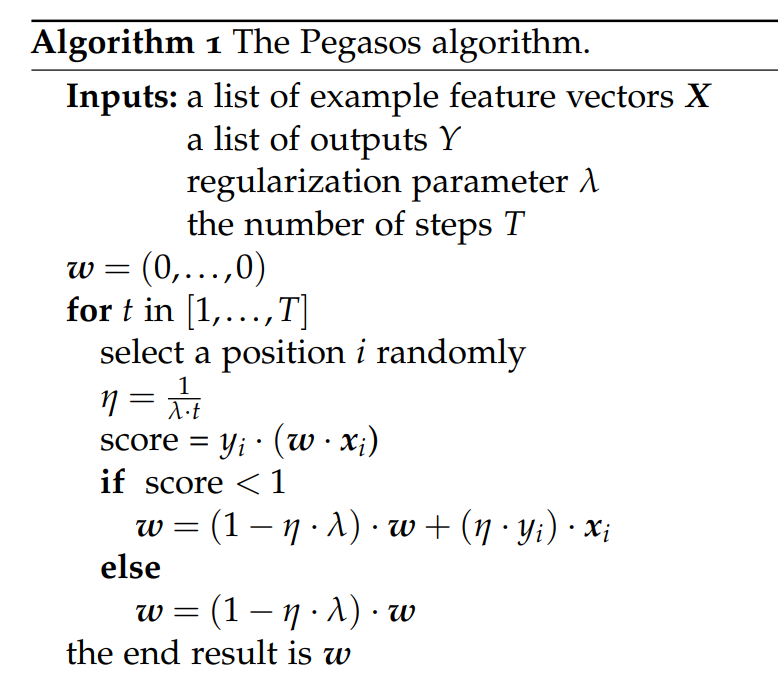
\includegraphics[height=5cm]{pic/pegasos-basic.png}
			\caption{Mô tả thuật toán Pegasos cơ bản bằng mã giả}
			\label{fig:svm}
		\end{figure}
	\end{frame}
	\subsubsection{Bước chiếu}
	\begin{frame}{Bước Chiếu}
		Giới hạn tập hợp các nghiệm khả thi trong phạm vi $ \frac{1}{\sqrt{\lambda}} $. Để thực hiện điều này, cập nhật $ \mathbf{w}_t $ sau mỗi vòng lặp:
		$$\mathbf{w}_{t+1} \leftarrow \min\left(1, \frac{1}{\sqrt{\lambda \|\mathbf{w}_{t+1}\|}}\right) \mathbf{w}_{t+1}.$$
	\end{frame}
	\subsubsection{Hàm mục tiêu và hàm mất mát Hinge}
	\begin{frame}{Hàm mục tiêu}
		Cần tìm vector trọng số $ \mathbf{w} $ để tối thiểu hóa hàm mục tiêu sau:
		$$f(\mathbf{w}, \mathbf{X}, \mathbf{Y}) = \frac{\lambda}{2} \cdot \|\mathbf{w}\|^2 + \frac{1}{|\mathbf{Y}|} \cdot \sum_{i} \text{Loss}(\mathbf{w}, \mathbf{x}_i, y_i)$$
		
		Đối với thuật toán SVM, hàm mất mát là hàm mất mát hinge:
		$$\text{Loss}(\mathbf{w}, \mathbf{x}_i, y_i) = \max(0, 1 - y_i \cdot (\mathbf{w} \cdot \mathbf{x}_i))$$
	\end{frame}
	\begin{frame}{Hàm mất mát Hinge}
		Hàm mất mát hinge có thể được viết rõ ràng hơn như sau:
		$$\text{Loss}(\mathbf{w}, \mathbf{x}_i, y_i) =       \begin{cases}           1 - y_i \cdot (\mathbf{w} \cdot \mathbf{x}_i) & \text{nếu } y_i \cdot (\mathbf{w} \cdot \mathbf{x}_i) < 1 \\          0 & \text{khác}      \end{cases}$$
		
		Điều mà Pegasos thực hiện là áp dụng một thuật toán tối ưu hóa để tìm $ \mathbf{w} $ tối thiểu hóa hàm mục tiêu $ f $:
		$$f(\mathbf{w}; A_t) = \frac{\lambda}{2} \|\mathbf{w}\|^2 + \frac{1}{k} \sum_{i \in A_t} \ell(\mathbf{w}; (\mathbf{x}_i, y_i)).$$
		với $ k $ là số lượng tập mini-batch.
	\end{frame}
	% Methods --- --- --- --- --- --- --- --- --- --- --- 
	\section{Cài đặt}
	\subsection{Tiền xử lý và chuẩn bị dữ liệu}
	\subsubsection{Load dữ liệu}
	\begin{frame}{Import thư viện}
		\begin{figure}
			\centering
			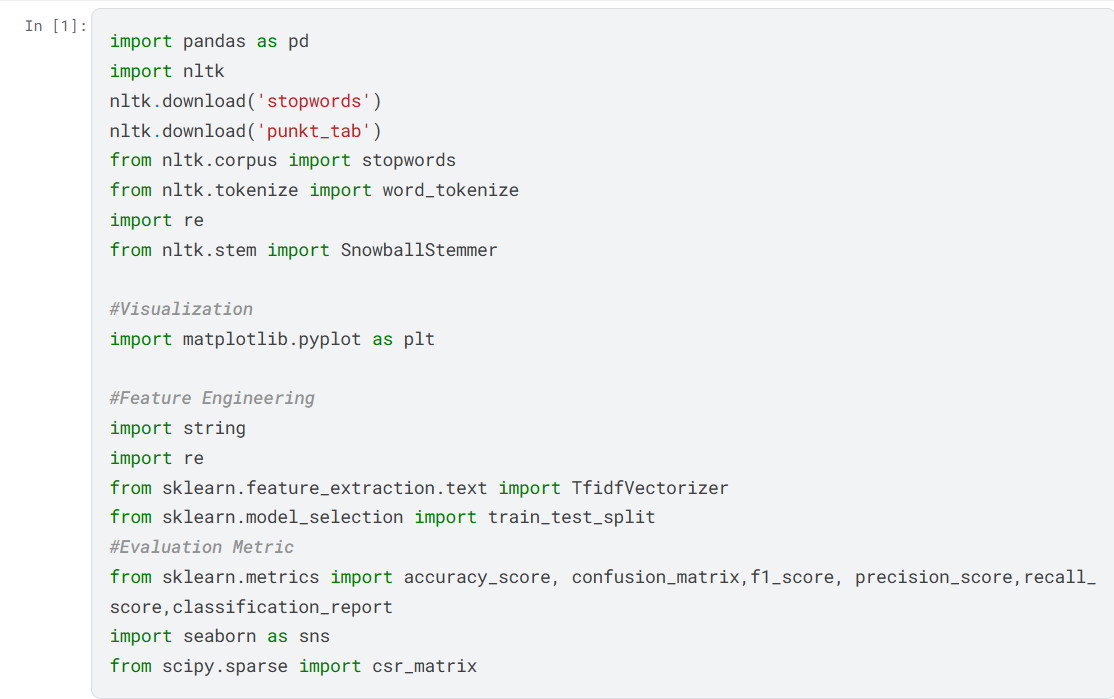
\includegraphics[width=0.7\linewidth]{pic/import-libraries.png}
			\label{fig:import-libraries}
		\end{figure}
	\end{frame}
	
	\begin{frame}{Load dữ liệu}
		\begin{figure}
			\centering
			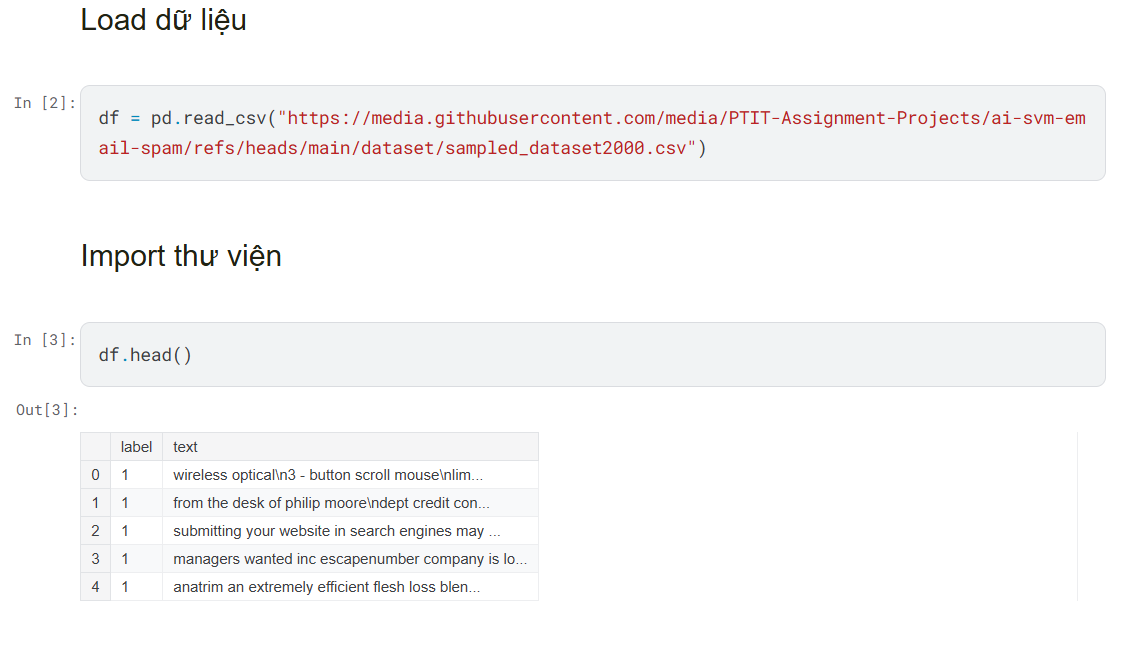
\includegraphics[width=0.8\linewidth]{pic/load-data.png}
			\label{fig:load-data}
		\end{figure}
	\end{frame}
	
	\subsubsection{Tiền xử lý dữ liệu}
	\begin{frame}{Xoá những ký tự đặc biệt và số}
		\begin{figure}
			\centering
			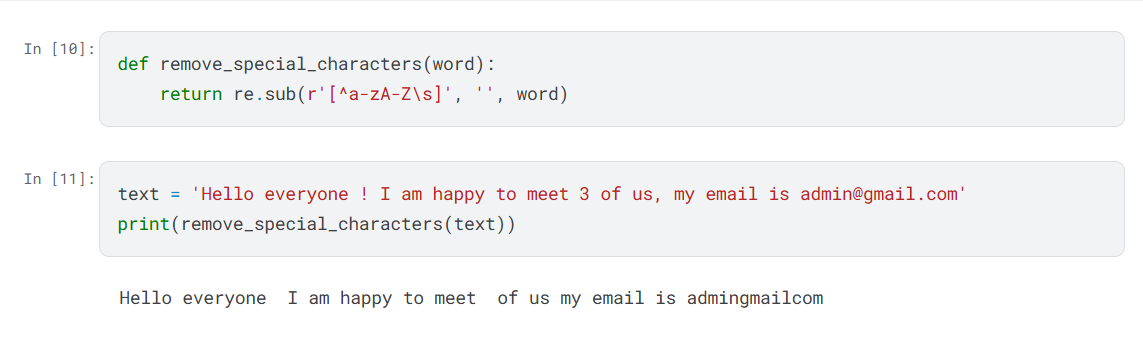
\includegraphics[width=1\linewidth]{pic/remove-special-char-num.png}
			\label{fig:remove-special-char-num}
		\end{figure}
	\end{frame}
	
	\begin{frame}{Xoá những stop words trong câu}
		\begin{figure}
			\centering
			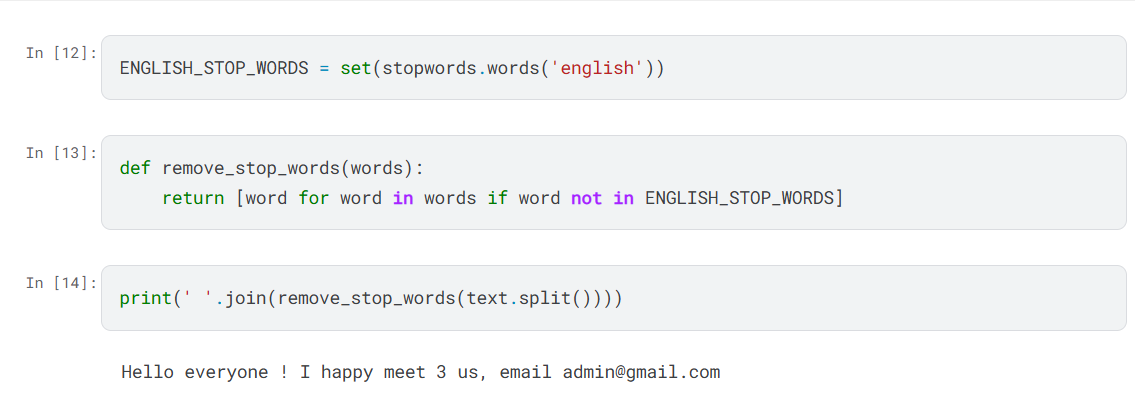
\includegraphics[width=1\linewidth]{pic/remove-stopwords.png}
			\label{fig:remove-stopwords}
		\end{figure}
	\end{frame}
	
	\begin{frame}{Xoá các link website trong câu}
		\begin{figure}
			\centering
			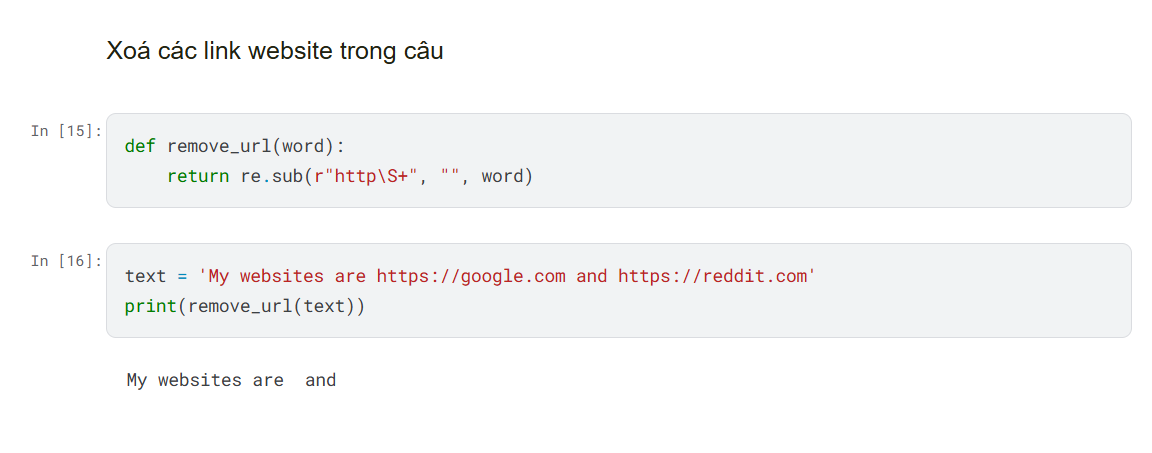
\includegraphics[width=1\linewidth]{pic/remove-link.png}
			\label{fig:remove-link}
		\end{figure}
	\end{frame}
	
	\begin{frame}{Áp dụng \texttt{word\_tokenize} vào data}
		\begin{figure}
			\centering
			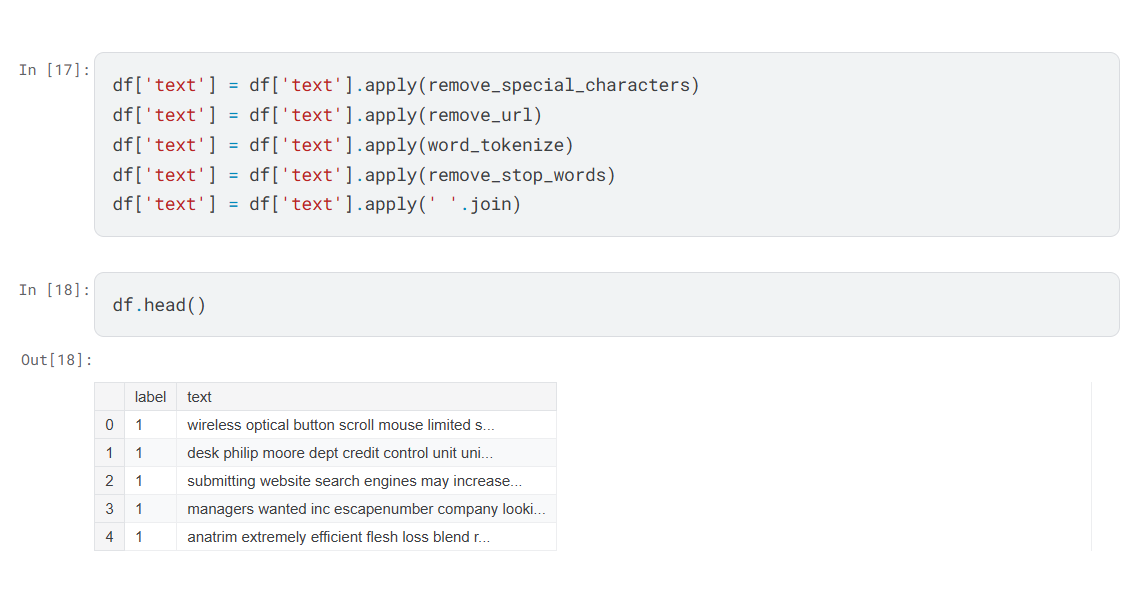
\includegraphics[width=1\linewidth]{pic/apply-tokenize.png}
			\label{fig:apply-tokenize}
		\end{figure}
	\end{frame}
	
	\begin{frame}{Snowball Stemmer}
		\begin{figure}
			\centering
			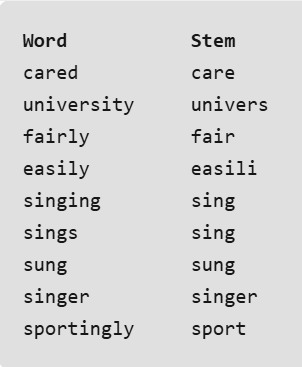
\includegraphics[width=0.4\linewidth]{pic/snowball-stemmer.png}
			\label{fig:snowball-stemmer}
		\end{figure}
	\end{frame}
	\begin{frame}{Snowball Stemmer}
		\begin{figure}
			\centering
			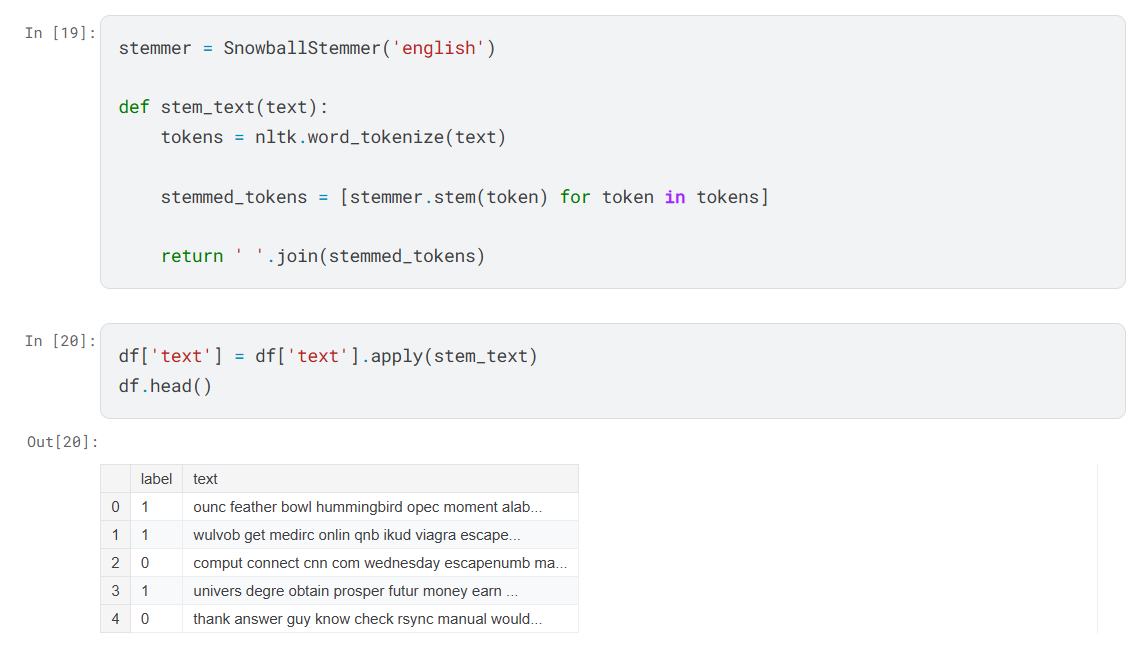
\includegraphics[width=0.8\linewidth]{pic/snowball-stemmer-apply.png}
			\label{fig:snowball-stemmer-apply}
		\end{figure}
	\end{frame}
	\begin{frame}{TF-IDF vectorization}
		\begin{figure}
			\centering
			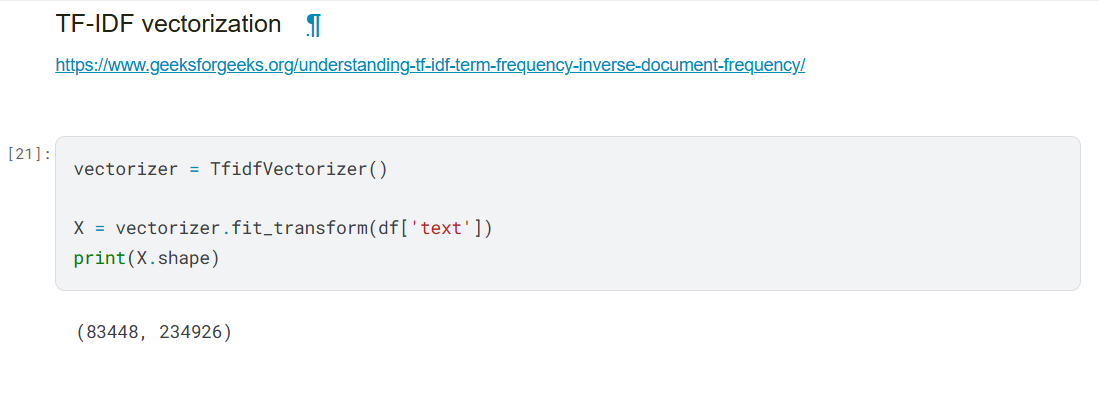
\includegraphics[width=1\linewidth]{pic/tfidf-apply.png}
			\label{fig:tfidf-apply}
		\end{figure}
	\end{frame}
	
	\subsubsection{Chuẩn bị dữ liêu}
	\begin{frame}{Chuẩn bị dữ liệu train và test}
		\begin{figure}
			\centering
			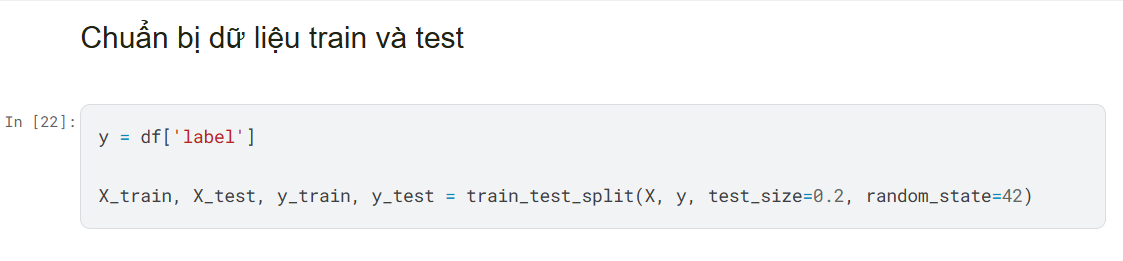
\includegraphics[width=1\linewidth]{pic/train_test_split.png}
			\label{fig:train-test-split}
		\end{figure}
	\end{frame}
	
	\subsection{Mô hình HardMarginSVM}
	\subsubsection{Viết mô hình HardMarginSVM}
	\begin{frame}{HardMarginSVM}
		\begin{figure}
			\centering
			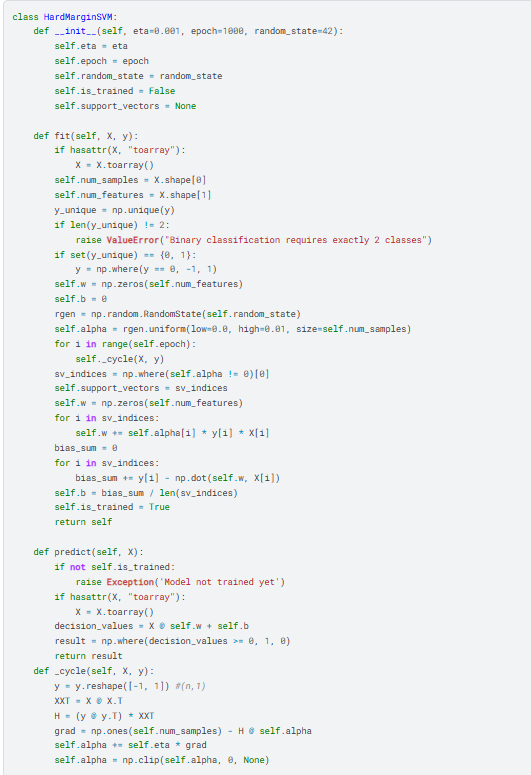
\includegraphics[width=0.5\linewidth]{pic/hard-margin-svm.png}
			\label{fig:hard-margin-svm}
		\end{figure}
	\end{frame}
	\subsubsection{Chạy thử trên tập dữ liệu 2000 mẫu}
	\begin{frame}{Kết quả}
		\begin{figure}
			\centering
			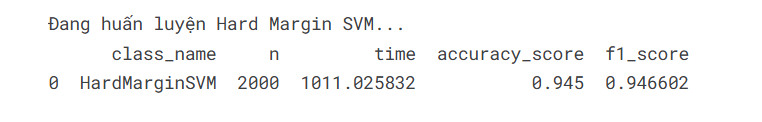
\includegraphics[width=1\linewidth]{pic/hardmargin-svm-result2000.png}
			\label{fig:hardmargin-svm-result2000}
		\end{figure}
	\end{frame}
	
	\subsubsection{Vấn đề}
	\begin{frame}{So sánh thời gian chạy với độ lớn bộ dữ liệu}
		\begin{figure}
			\centering
			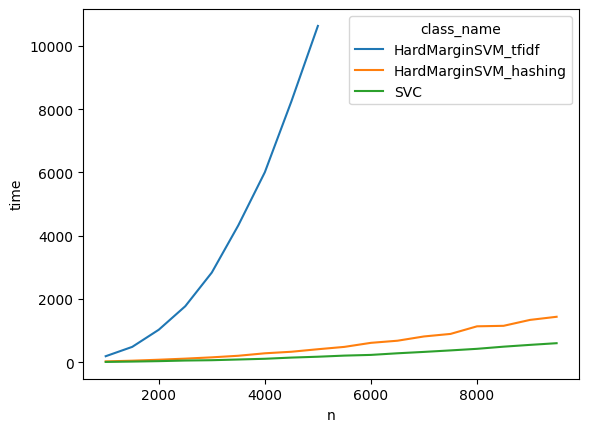
\includegraphics[width=0.6\linewidth]{pic/n-time-hardmargin-svm.png}
			\label{fig:n-time-hardmargin-svm}
		\end{figure}
	\end{frame}
	
	\begin{frame}{So sánh độ lớn bộ dữ liệu với độ chính xác}
		\begin{figure}
			\centering
			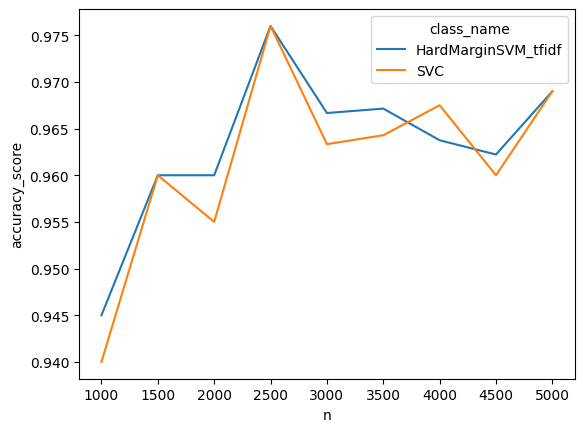
\includegraphics[width=0.6\linewidth]{pic/n-acc-hardmargin-svm.png}
			\label{fig:n-acc-hardmargin-svm}
		\end{figure}
	\end{frame}
	
	\subsection{Mô hình SVM tối ưu bởi thuật toán Pegasos}
	\subsubsection{Viết mô hình}
	\begin{frame}{SVM với thuật toán Pegasos}
		\begin{figure}
			\centering
			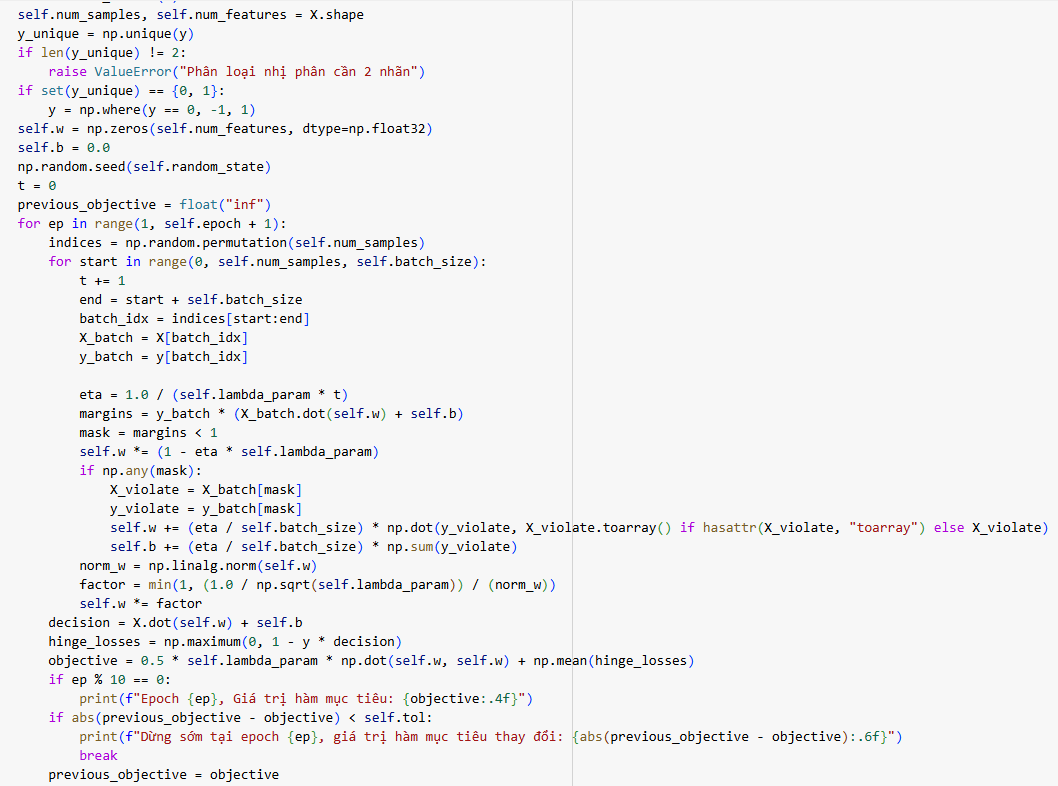
\includegraphics[width=0.6\linewidth]{pic/svm-pegasus.png}
			\label{fig:svm-pegasus}
		\end{figure}
	\end{frame}
	\subsubsection{Chạy thử trên tập dữ liệu}
	\begin{frame}{Kết quả}
		\begin{figure}
			\centering
			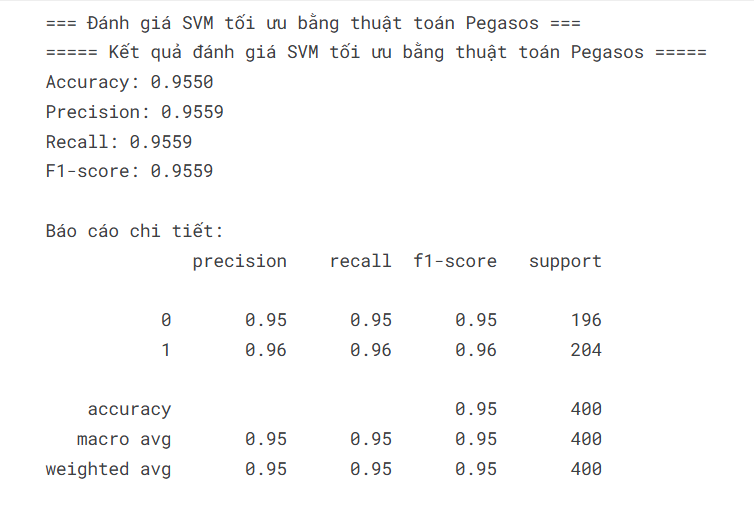
\includegraphics[width=0.7\linewidth]{pic/svm-pegasos-result2000.png}
			\label{fig:svm-pegasos-result2000}
		\end{figure}
	\end{frame}
	\subsubsection{So sánh với HardMarginSVM}
	\begin{frame}{So sánh thời gian chạy với độ lớn bộ dữ liệu}
		\begin{figure}
			\centering
			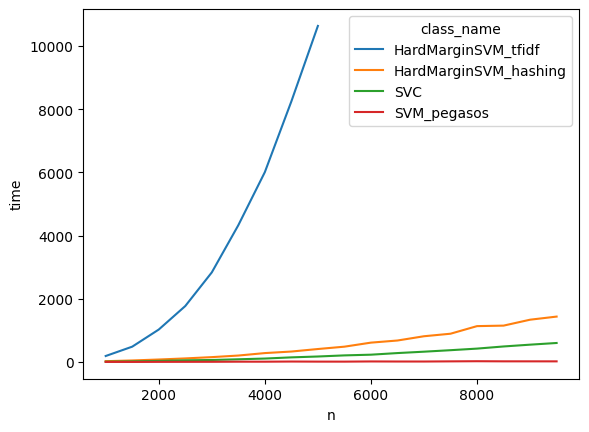
\includegraphics[width=0.6\linewidth]{pic/hardmargin-vs-pegasos-n-time.png}
			\label{fig:hardmargin-vs-pegasos-n-time.}
		\end{figure}
	\end{frame}
	
	\begin{frame}{So sánh độ lớn bộ dữ liệu với độ chính xác}
		\begin{figure}
			\centering
			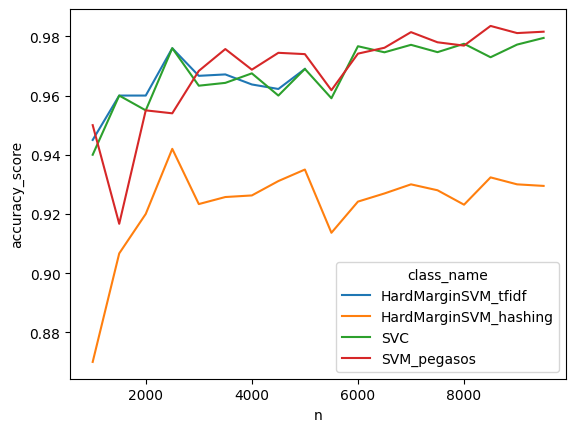
\includegraphics[width=0.6\linewidth]{pic/hardmargin-vs-pegasos-n-vs-acc.png}
			\label{fig:hardmargin-vs-pegasos-n-vs-acc}
		\end{figure}
	\end{frame}
	\subsection{Chạy với bộ dữ liệu ban đầu và lưu mô hình}
	\begin{frame}{Kết quả}
		\begin{figure}
			\centering
			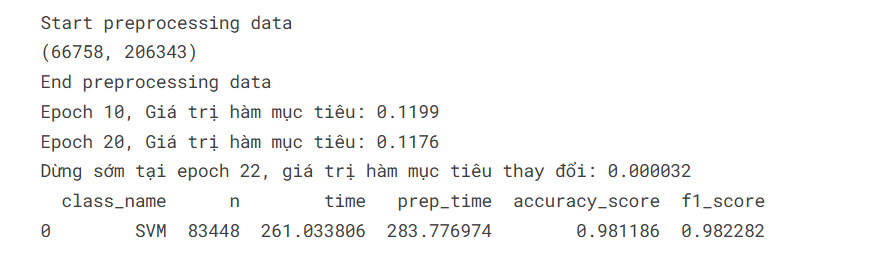
\includegraphics[width=1\linewidth]{pic/svm-pegasos-result-full.png}
			\label{fig:svm-pegasos-result-full}
		\end{figure}
	\end{frame}
	
	\begin{frame}{Lưu mô hình và vectorizer}
		\begin{figure}
			\centering
			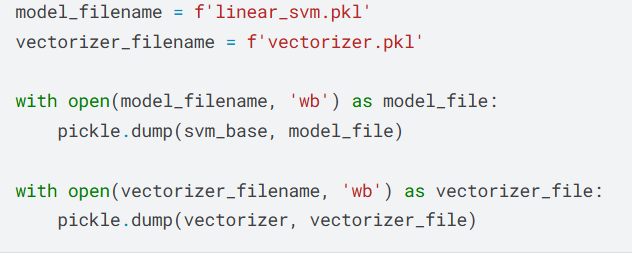
\includegraphics[width=1\linewidth]{pic/save-model-vectorizer.png}
			\label{fig:save-model-vectorizer}
		\end{figure}
	\end{frame}
	
	
	
	% Results --- --- --- --- --- --- --- --- --- --- --- 
	\section{Triển khai và demo}
	\subsection{Mô tả cách triển khai}
	\begin{frame}{Mô tả cách triển khai}
		\begin{itemize}
			\item Sử dụng streamlit để tạo giao diện trên web và xử lý phần mô hình
			\item Load 2 file nhị phân model và vectorizer để tiến hành dự đoán đầu vào
			\item Sử dụng docker để đóng gói
		\end{itemize}
		
	\end{frame}
	\begin{frame}{Sơ đồ tổng quan}
		\begin{figure}
			\centering
			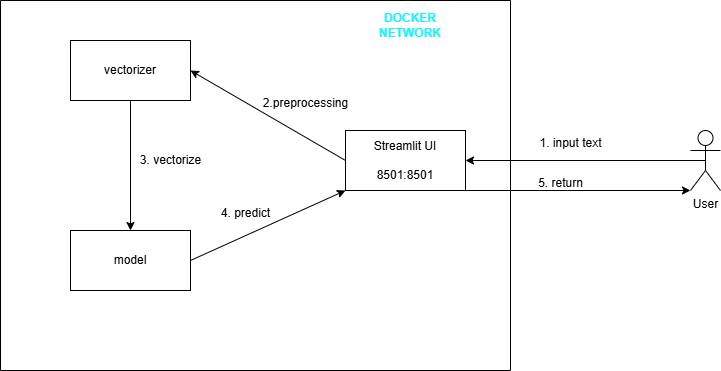
\includegraphics[width=0.8\linewidth]{pic/demo-ai-sys.png}
			\label{fig:demo-ai-sys}
		\end{figure}
	\end{frame}
	\begin{frame}{Giao diện demo spam}
		\begin{figure}
			\centering
			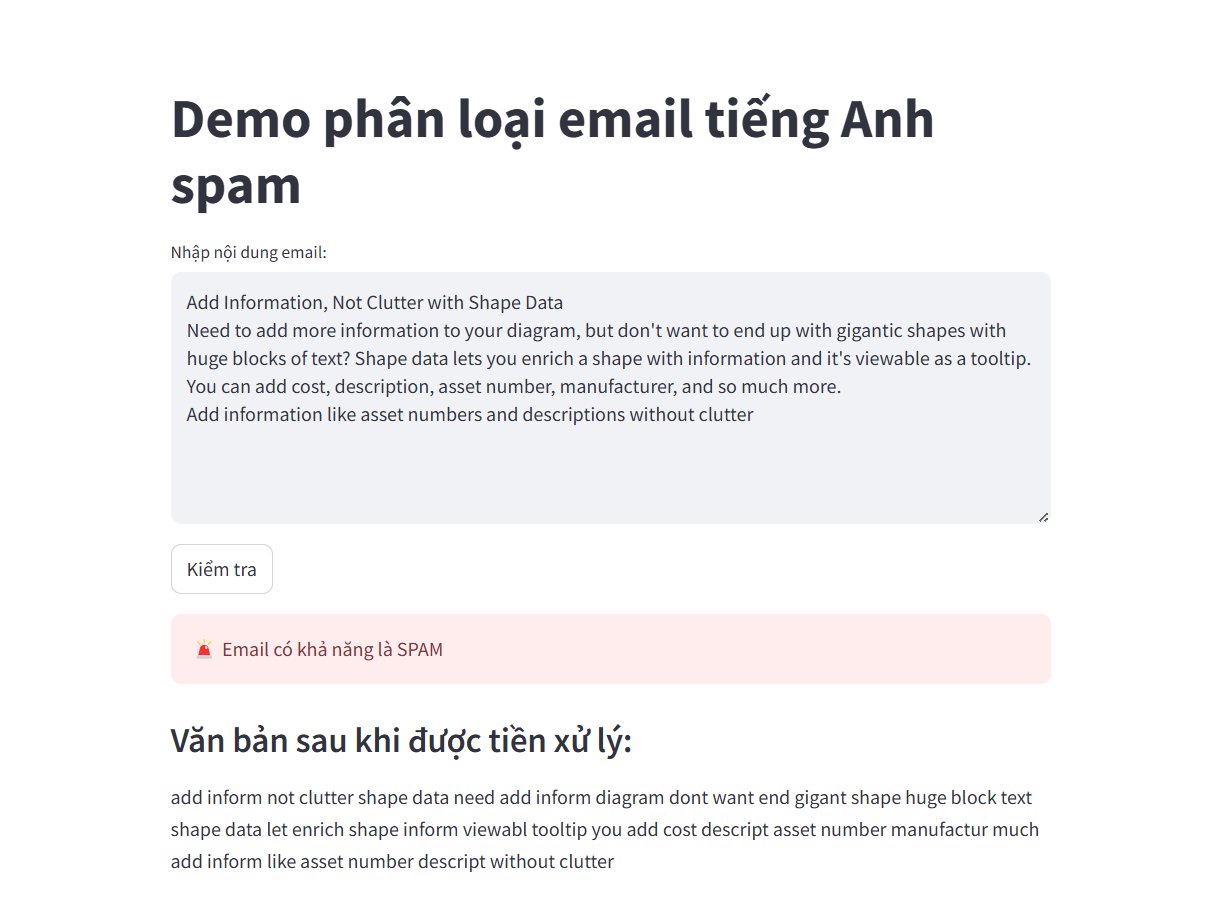
\includegraphics[width=0.6\linewidth]{pic/demo-spam.png}
			\label{fig:demo-spam}
		\end{figure}
	\end{frame}
	\begin{frame}{Giao diện demo không spam}
		\begin{figure}
			\centering
			
\includegraphics[width=0.6\linewidth]{pic/demo-not-spam.png}
			\label{fig:demo-not-spam}
		\end{figure}
	\end{frame}
	
	% --- Thank you slide ---
	\begin{frame}
		\begin{center}
			{ Cảm ơn cô đã lắng nghe!}
			\vspace{1cm}
			
		\end{center}
	\end{frame}
	
\end{document}